% LuaLaTeX文書; 文字コードはUTF-8
\documentclass[unicode,12pt]{beamer}% 'unicode'が必要
\usepackage{luatexja}% 日本語したい
\usepackage[ipaex]{luatexja-preset}% IPAexフォントしたい
\renewcommand{\kanjifamilydefault}{\gtdefault}% 既定をゴシック体に

\usepackage{amssymb,amsmath,ascmac}
\usepackage{derivative}

\usepackage{multirow}
\usepackage{bm}

\graphicspath{{../fig/}}

\usepackage{animate}
\usepackage{tikz}
\usepackage{xparse}

%目次スライド
\AtBeginSection[]{
  \frame{\tableofcontents[currentsection]}
}
%アペンディックスのページ番号除去
\newcommand{\backupbegin}{
\newcounter{framenumberappendix}
\setcounter{framenumberappendix}{\value{framenumber}}
}
\newcommand{\backupend}{
\addtocounter{framenumberappendix}{-\value{framenumber}}
\addtocounter{framenumber}{\value{framenumberappendix}} 
}

%%%%%%%%%%%  theme  %%%%%%%%%%%
\usetheme{Copenhagen}
% \usetheme{Metropolis}
% \usetheme{CambridgeUS}
% \usetheme{Berlin}

%%%%%%%%%%%  inner theme  %%%%%%%%%%%
% \useinnertheme{default}

% %%%%%%%%%%%  outer theme  %%%%%%%%%%%
\useoutertheme{default}
% \useoutertheme{infolines}

%%%%%%%%%%%  color theme  %%%%%%%%%%%
%\usecolortheme{structure}

%%%%%%%%%%%  font theme  %%%%%%%%%%%
\usefonttheme{professionalfonts}
%\usefonttheme{default}

%%%%%%%%%%%  degree of transparency  %%%%%%%%%%%
%\setbeamercovered{transparent=30}

% \setbeamertemplate{items}[default]

%%%%%%%%%%%  numbering  %%%%%%%%%%%
% \setbeamertemplate{numbered}
\setbeamertemplate{navigation symbols}{}
\setbeamertemplate{footline}[frame number]


\title{粘着・剥離の基礎と\\タッキファイヤーの働き}
\subtitle{~ 第三章「表面張力、相溶性、混合状態の理解」 ~}
\author[東亞合成 佐々木]{佐々木 裕\thanks{hiroshi\_sasaki@mail.toagosei.co.jp}}
\institute[東亞合成]{東亞合成株式会社}
\date{2024/2/15}

\begin{document}

%%%%%
% 1 P
%%%%%
\maketitle

\begin{frame} 
    \tableofcontents[]
\end{frame} 

\section{表面張力とはなにか?}

\subsection{表面張力の古典的な理解}
\begin{frame}
	\frametitle{表面張力の古典的な理解}
	\begin{block}{自然現象の観察から}
		\begin{itemize}
			\item 葉の上の水滴の形が丸くなること
			\item コップいっぱいの水がフチを越えて盛り上がること
			\item 一円玉が水に浮かぶこと
		\end{itemize}
		\begin{columns}[c, onlytextwidth]
			\column{.33\linewidth}
			\centering
			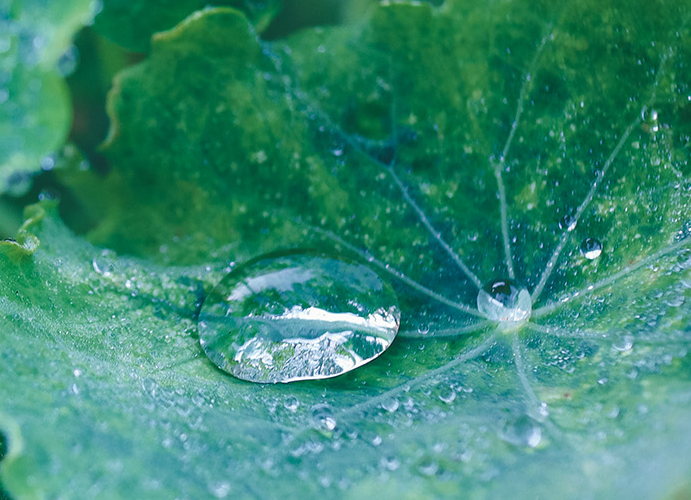
\includegraphics[width=.6\textwidth]{waterdrop.png}
			\column{.33\linewidth}
			\centering
			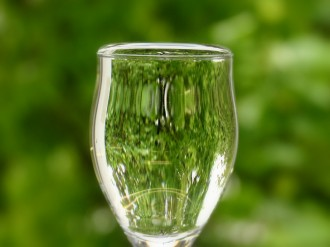
\includegraphics[width=.6\textwidth]{hyoumen_cup.jpg}
			\column{.33\linewidth}
			\centering
			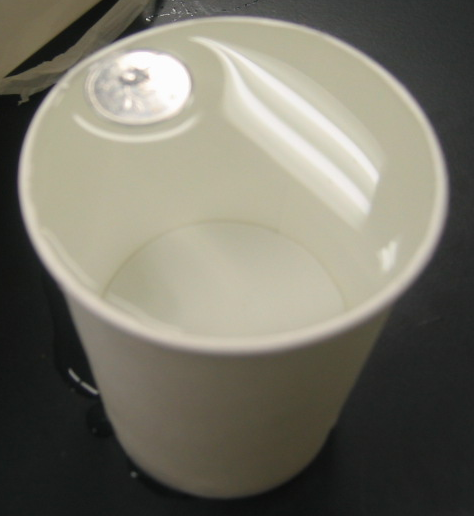
\includegraphics[width=.41\textwidth]{hyoumen_1.png}
		\end{columns}
	\end{block}

	\begin{exampleblock}{上記の現象から、力として理解}
		\begin{itemize}
			\item 液体の表面に張り詰めた力をイメージ
			\item 表面を小さくしようとする力とも考えられた
			\item 「表面の1cmを横切る力 (dyne/cm=mN/m)」と定義
		\end{itemize}
	\end{exampleblock}
\end{frame}

\begin{frame}
	\frametitle{Young 式のイメージ}
	\begin{block}{Young 式は、力の釣り合いを考えたもの}
		\begin{columns}[c, onlytextwidth]
			\column{.48\linewidth}
			\begin{align*}
				\gamma_{SV} = \gamma_{LV} \cos \theta + \gamma_{SL}
			\end{align*}
			\column{.48\linewidth}
			\begin{itemize}
				\item $\gamma_{SV}$ は固体⇔空気
				\item $\gamma_{LV}$ は液体⇔空気
				\item $\gamma_{SL}$ は液体⇔固体
			\end{itemize}
		\end{columns}
		
		\vspace{2mm}
		\begin{itemize}
			% \item $\gamma_{SV}$ は固体表面と空気との間での力
			% \item $\gamma_{LV}$ は液体と空気との間の力
			% \item $\gamma_{SL}$ は液体と固体との間の力
			\item 液滴を縮める力($\gamma_{LV} \cos \theta + \gamma_{SL}$)と広げる力($\gamma_{SV}$)の釣り合い
		\end{itemize}

		\centering
			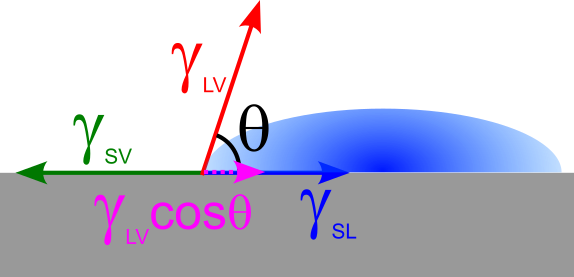
\includegraphics[width=.45\textwidth]{young.png}
	\end{block}
\end{frame}
\subsection{表面張力の現代的理解}
\begin{frame}
	\frametitle{仕事量としての解釈}
	\vspace{-3mm}
	\begin{columns}[c, onlytextwidth]
		\column{.65\linewidth}
				\begin{itemize}
					\item コの字形の枠と可動する棒の間に張られた液体の膜を考える。
					\item 可動する棒には表面に平行に、膜を収縮させる向きに力 $F$ が働く。
					\item この力と釣り合うように微小長さ $\Delta x$ だけ引き伸ばす。
					\item \alert{液表面を単位面積広げる仕事量}を表面エネルギーと定義
				\end{itemize}
		\column{.32\linewidth}
		\centering
		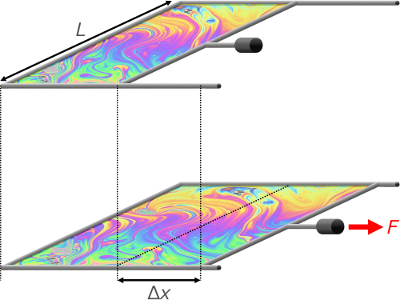
\includegraphics[width=\textwidth]{maxwells-frame.jpg}

		\vspace{2mm}
		Maxwell の枠
	\end{columns}
	
	\only<1>{
		\begin{block}{表面エネルギーの定義}
			\vspace{-5mm}
			\begin{align*}
				\text{表面エネルギー} 
				&= \text{液表面を単位面積広げるエネルギー} \\
				% &= \dfrac{\text{必要な力 $\times$ 距離}}{\text{拡張面積}}\\
				&= \dfrac{\Delta x\cdot F}{\Delta x\cdot L }
			\end{align*}
		\end{block}
	}

	\uncover<2>{
		\begin{alertblock}{現代的な表面張力の理解}
			\begin{columns}[c, onlytextwidth]
				\column{.75\linewidth}
				\begin{itemize}
					\item 単位長さあたりの力 (N/m) ではなく
					\item 単位面積あたりの仕事量 (J/m$^2$)
				\end{itemize}
				\column{.22\linewidth}
					\alert{同じ次元}
			\end{columns}
		\end{alertblock}
		}
\end{frame}

\begin{frame}
	\frametitle{表面張力(表面エネルギー)の分子論的な理解}

	\begin{columns}[c, onlytextwidth]
		\column{.7\linewidth}
			\begin{itemize}
				\item 液体内部の一分子に着目すると、
				\begin{itemize}
					\item 周囲を他の分子に取り囲まれている
					\item \textcolor{red}{相互に分子間力}を及ぼし合っている
					\item エネルギー的に低い安定状態
				\end{itemize}
				\item 表面の分子は上に分子が存在しない
				\begin{itemize}
					\item 内部の分子よりも高エネルギー状態
					\item \textcolor{blue}{表面を小さくしたい力が発生}
					\item 他の分子に相互作用しうる\textcolor{red}{過剰な\\エネルギー}を持っている
					\item これを表面エネルギーとして理解すれば良い
				\end{itemize}
			\end{itemize}
		\column{.28\linewidth}
		\centering
		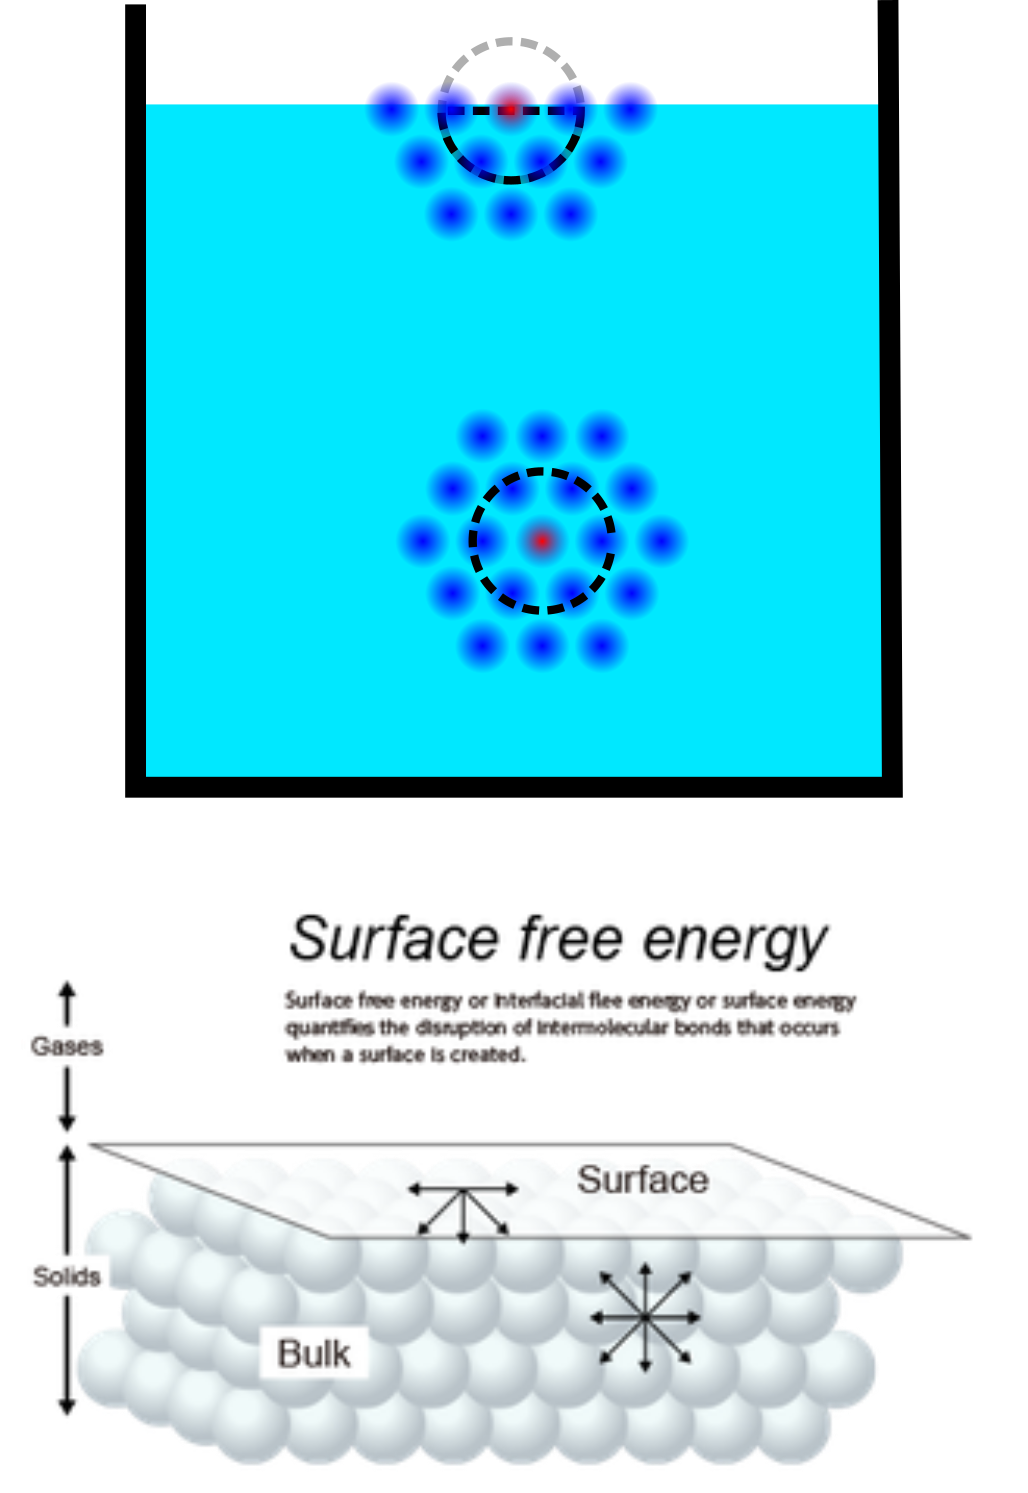
\includegraphics[width=\textwidth]{surface.png}
	\end{columns}
\end{frame}

\subsection{濡れと接着仕事}
\begin{frame}
	\frametitle{濡れのイメージ}
	
		\begin{block}{接触角 $\theta$ で濡れを理解}
			\begin{columns}[c, onlytextwidth]
				\column{.6\linewidth}
					\begin{itemize}
						\item $\theta = 90^{o}$: $\gamma_{LV}$ の寄与はない。
						\item $\theta < 90^{o}$: 固体は気体と接するよりも液体の方が好き。
						\item $\theta > 90^{o}$: 固体は気体と接するほうが居心地がいい。
					\end{itemize}
				\column{.35\linewidth}
				\centering
				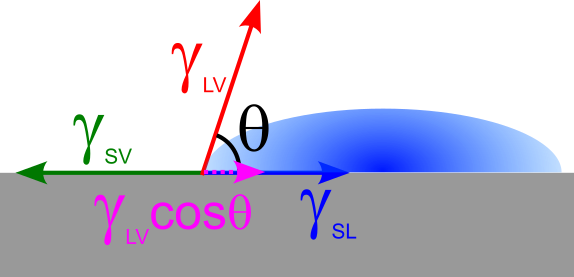
\includegraphics[width=\textwidth]{young.png}
			\end{columns}
		\end{block}
	\vspace{5mm}
	\centering
			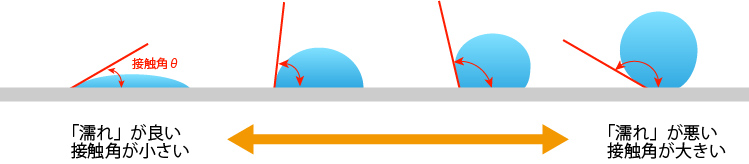
\includegraphics[width=\textwidth]{wetting.png}
\end{frame}


\begin{frame}
	\frametitle{Dupr\'{e} の接着仕事}
		\begin{columns}[c, onlytextwidth]
			\column{.7\linewidth}
				\begin{itemize}
					\item 物体1と2が界面で接している状態
					\item 引き離すと新たに2つの表面が生成
					\item 離脱前後での界面エネルギーの差が\alert{分離に必要なエネルギー}となる。
					\item これを\alert{接着仕事}と考える。
				\end{itemize}

				\vspace{-10mm}
				\begin{align*}
					W_{a} = \gamma_1 + \gamma_2 - \gamma_{12}
				\end{align*}
			\column{.28\linewidth}
			\centering
			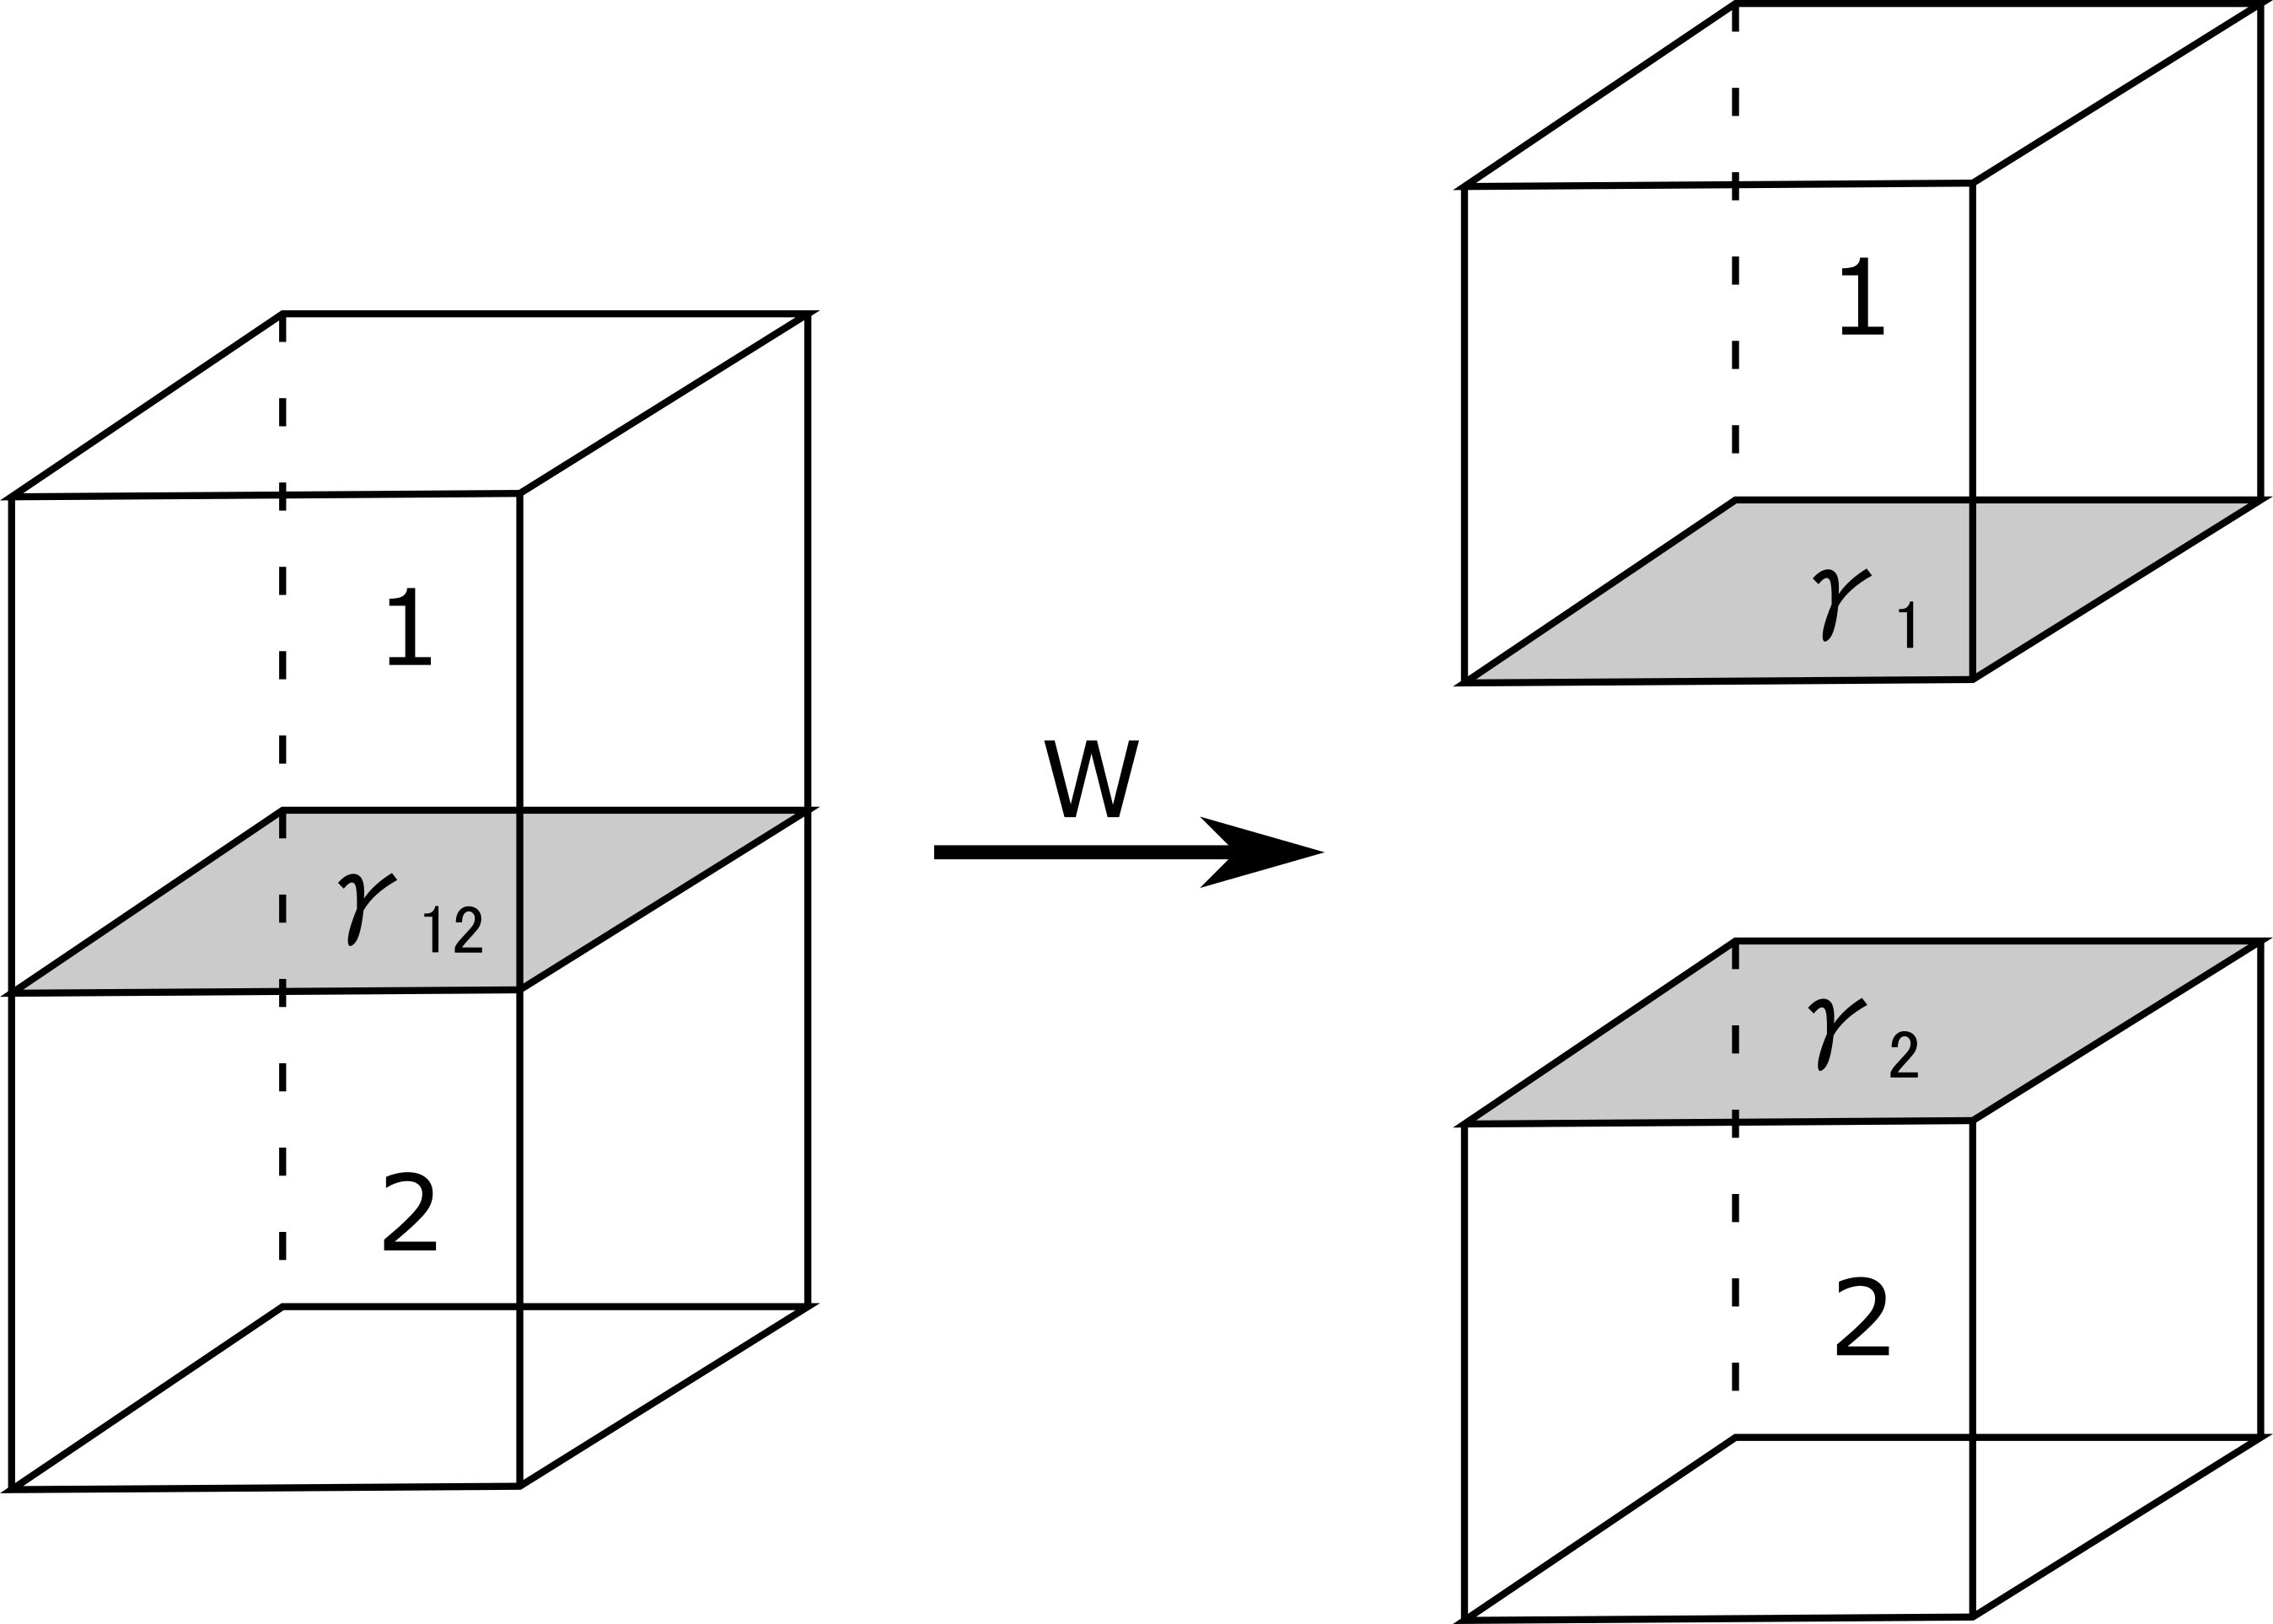
\includegraphics[width=\textwidth]{settyaku_shigoto.png}
		\end{columns}

		\pause
		\begin{alertblock}{Young-Dupr\'{e} の式}
			一方が液体であった場合、Young 式を用いて、
			\vspace{-5mm}
			\begin{align*}
				W_{a} &= \gamma_{LV} + \gamma_{SV} - \gamma_{SL} \\
				&= \gamma_{LV} + (\gamma_{LV} \cos \theta + \gamma_{SL}) - \gamma_{SL} \\
				&= \gamma_{LV}(1 + \cos \theta)
			\end{align*}
		\end{alertblock}
\end{frame}

\begin{frame}
	\frametitle{「表面張力と濡れ」のまとめ}
        \begin{boxnote}
            \vspace{-3mm}
            \begin{itemize}
                \item 表面張力の古典的理解
                    \begin{itemize}
                        \item 液体の表面に張り詰めた力をイメージ
						\item 表面を小さくしようとする力とも
						\item Young 式は力の釣り合いを考えた
                    \end{itemize} 
				\item 現代的には仕事量として理解
                    \begin{itemize}
                        \item 表面エネルギーとして解釈
                        \item 分子の相互作用が気液界面でバランスが変化
                    \end{itemize}
                \item 濡れと接着仕事
                    \begin{itemize}
                        \item 接触角$\theta$で濡れを理解
                        \item 接着仕事にも繋がりやすい
                    \end{itemize} 
            \end{itemize}
        \end{boxnote}
\end{frame}

\section{相溶性と溶解度パラメタ}
\subsection{自由エネルギーによる系の記述}
\begin{frame}\frametitle{自由エネルギーによる系の記述}
	\begin{block}{物質の安定な状態とは?} 
		\begin{itemize}
			\item 熱力学によれば、「自由エネルギーが最小となる状態」
			% \item 系の\alert{平衡構造}を記述可能
			\item 以下 Gibbs の自由エネルギー $G$ の表式
				\begin{itemize}
					\item エンタルピー:内部エネルギーと定圧下での変化に伴う仕事との和
					\item エントロピー:系の変化に伴う自由度の変化を表す指標
				\end{itemize}
				\vspace{-.5\baselineskip}
				\begin{align*}
					G &= \color{blue}H\color{black} - \color{green}TS\color{black} \notag \\
						&= \text{\color{blue}エンタルピー項\color{black}} - \text{\color{green}エントロピー項\color{black}}
				\end{align*}
			\item \alert{自由エネルギーが減少する方向に物事は進む。}\\
			ただし、外的な作用があればそうなるとは限らないが。
		\end{itemize}
	\end{block}
\end{frame}

\subsection{異種の液体が溶け合うということは?}
\begin{frame}
	\frametitle{異種の液体が溶け合うということは?}
	\begin{exampleblock}{混合の自由エネルギー変化 $\Delta G$}
		A, B の二相を混合する際の自由エネルギー変化は?
		\vspace{-.5\baselineskip}
		\begin{align*}
			\Delta G 
			% &= \text{混合後の自由エネルギー} - \text{混合前の自由エネルギーの和} \\
			&= G_{mix} - (G_A + G_B) \\
			&= \text{エンタルピー変化量} - T \times \text{エントロピー変化量} \\
			&= \Delta H -T \Delta S
		\end{align*}
	\end{exampleblock}
	
	\begin{block}{溶け合うということは?}
		\begin{itemize}
			\item 混合で自由エネルギーが低下⇒安定な状態
			\item 溶解の条件:$\Delta G < 0$
		\end{itemize}
	\end{block}
\end{frame}

\subsection{溶解度パラメタ}
\begin{frame}
	\frametitle{溶解度パラメタ Solubility Parameter}
		\begin{block}{Hildebrand の溶解度パラメタ: SP 値 $\delta$}
			\begin{itemize}
				\item 似たもの同士が溶けやすいという経験則
				\item Hildebrand が\textcolor{red}{正則溶液(単純化した理想状態)}で提唱
				\begin{itemize}
					\item 理想溶液;混合によっても、エンタルピー、エントロピーともに変化しない
					⇔混合で溶解
					\item 正則溶液;エントロピーは変化しないが、エンタルピー変化を考慮
				\end{itemize}
				\vspace{-.5\baselineskip}
				\begin{align*}
					\Delta H &= \phi_A \phi_B V (\delta_A -\delta_B)^2 \\
					\text{where }& \phi_A, \phi_B \text{; volume fraction}\\
					& V \text{; Volume of System}
				\end{align*}
				\item SP 値が近いものが相溶する(実際には例外も多い)
			\end{itemize}
		\end{block}
\end{frame}

\begin{frame}
	\frametitle{溶解度パラメタ Solubility Parameter}
		\begin{block}{Hildebrand の溶解度パラメタ: SP 値 $\delta$}
			\vspace{-1\baselineskip}
			\begin{align*}
				\Delta H &= \phi_A \phi_B V (\delta_A -\delta_B)^2 \\
				\text{where }& \phi_A, \phi_B \text{; volume fraction}\\
				& V \text{; Volume of System}
			\end{align*}
			\vspace{-1\baselineskip}
			\begin{itemize}
				\item 溶解度の目安となるパラメタを分子間力から定義
				\vspace{-.5\baselineskip}
				\begin{align*}
					\delta = (\text{凝集エネルギー密度: CED})^{1/2} \\
				\end{align*}
			\end{itemize}
			\vspace{-8mm}
			\centering
				\only<2>{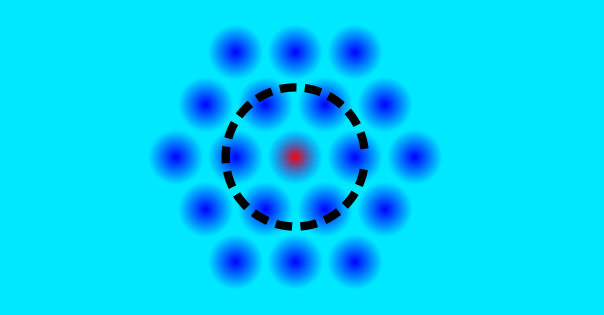
\includegraphics[width=.35\textwidth]{CED.png}}
				\uncover<3>{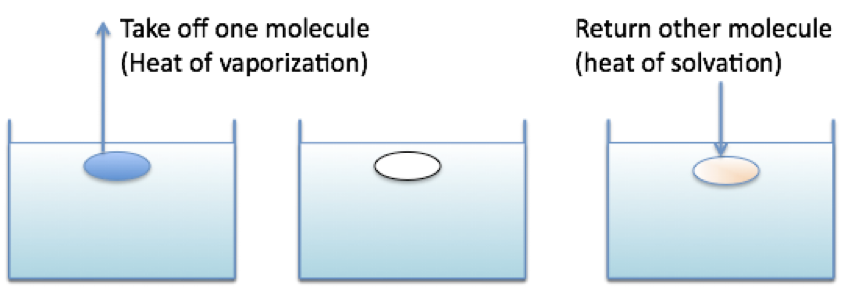
\includegraphics[width=.65\textwidth]{SP_BasicConsept.png}}
		\end{block}
\end{frame}

\begin{frame}
	\frametitle{凝集エネルギー密度}
		\begin{exampleblock}{凝集エネルギー密度(CED; Cohesive Energy Density)}
			\begin{itemize}
				\item 単位体積あたりの蒸発に必要なエネルギーのイメージ
				\item 凝集状態にある分子、原子を無限遠にまで引き離すのに必要なエネルギーを体積で割ったもの
				\item 蒸発エンタルピー $\Delta H_v$ から蒸発に必要な仕事(RT)を差引く
			\end{itemize}
			\vspace{-1\baselineskip}
			\begin{align*}
				&\text{CED} = \dfrac{\Delta H_v - RT}{\nu}\\
				&\text{$\Delta H_v$ は蒸発エンタルピー、}\\
				&\text{$R$ は気体定数、$T$ は温度、$\nu$ はモル体積}
			\end{align*}
		\end{exampleblock}
\end{frame}

\begin{frame}
	\frametitle{「相溶性と溶解度パラメタ」のまとめ}
        \begin{boxnote}
            \vspace{-3mm}
            \begin{itemize}
                \item 自由エネルギーによる系の記述
                    \begin{itemize}
                        \item 自由エネルギーはエンタルピーとエントロピーとで記述される
						\item 自由エネルギーが減少する方向に物事は進む
						\item 正確には平衡状態で自由エネルギーが最小化
                    \end{itemize} 
                \item 異種の液体が溶け合うためには
                    \begin{itemize}
                        \item 混合による自由エネルギー変化を考える
                        \item 単純化した正則溶液で Hildebrand が溶解度パラメタ
                        \item 溶解度パラメタが近いものが相溶する
                        \item 溶解度パラメタを凝集エネルギーから定義
                    \end{itemize} 
            \end{itemize}
        \end{boxnote}
\end{frame}

\section{混合状態を自由エネルギーから理解}
\subsection{相溶と非相溶}
\begin{frame}
	\frametitle{相溶と非相溶}
	\begin{columns}[c, onlytextwidth]
		\column{.7\linewidth}
			\begin{itemize}
				\item 「水と油」は非相溶
				\item 互いにまったく溶け合わないの?
				\begin{itemize}
					\item 水層中の油は 0 なの?
					\item 油層中の水は?
				\end{itemize}
				\item 溶ける溶けないの議論では不十分
			\end{itemize}
		\column{.3\linewidth}
				\centering
					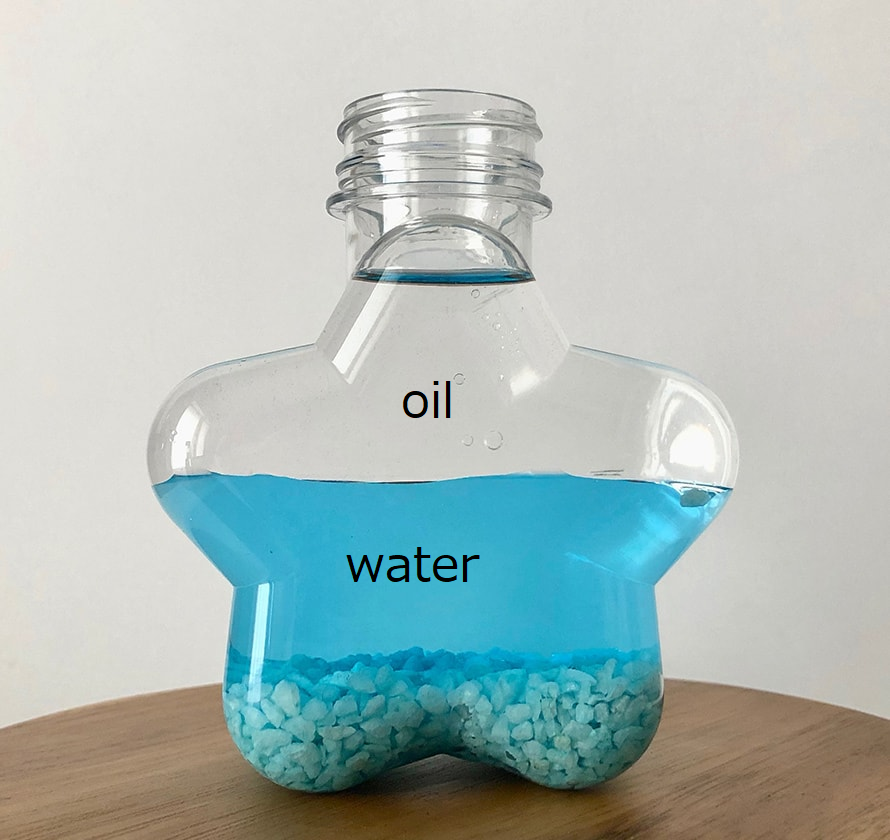
\includegraphics[width=\textwidth]{oil_water.png}
	\end{columns}

	\pause
	\begin{exampleblock}{「層」と「相」}
		\begin{itemize}
			\item 層(layer):一般に用いられる状態を表す言葉\\
			厚みをもつ構造体を表す
			\item 相(phase):\alert{熱力学で用いる用語}\\
			\alert{組成や物理状態が均一}となるような物質の形態
		\end{itemize}
	\end{exampleblock}

	\pause
	\Large
	\centering
	\alert{「熱力学的にもう少しの考察が必要!」}
\end{frame}

\subsection{自由エネルギーの濃度依存性について}
\begin{frame}
	\frametitle{自由エネルギーの濃度依存性について}
		\vspace{-3mm}
		\begin{block}{対象となる系の条件}
			\begin{itemize}
				\item 化学的な性状の異なる、A成分とB成分を混合
				\item 温度、体積、粒子数が一定で系の体積は$V$
				\item A成分の体積分率を $\phi$ とし、B 成分は $1-\phi$
				\item \alert{仮想的に任意の組成で一様に混合可能}とする
				% \item 混合の自由エネルギーは、$\phi$ の関数
				\item 自由エネルギー密度 $f(\phi)=\dfrac{F_{uni}(\phi)}{V}$ で状態を評価
			\end{itemize}
		\end{block}
		\vspace{-3mm}
		\begin{alertblock}{自由エネルギー曲線}
			\begin{itemize}
				\item $f(\phi)$ は $\phi$ により定まる $(\phi, f(\phi) )$ 平面上の曲線
				\item 系中の一部分の局所的な状態を考える
				\begin{itemize}
					\item 濃度ゆらぎが生じて一様状態から変化したとき、
					\item 局所的な状態は $f_{local}$ と $f(\phi)$ との大小関係から決まる
				\end{itemize}
			\end{itemize}
		\end{alertblock}
\end{frame}

\begin{frame}
	\frametitle{二相分離を考えてみると}
		\begin{itemize}
		\item 一様混合
		\begin{itemize}
			\item \alert{「仕込み濃度の組成」で一様}に存在。
			\end{itemize}
		\item 二相分離
		\begin{itemize}
			 \item $\alpha$相と$\beta$相との\alert{二つの相}に分離。
			 \item それぞれの相において、\\各成分が\alert{「仕込み濃度とは異なる濃度で一様に混合」}
			 \item 界面は無視する。
		\end{itemize}
	\end{itemize}
	\begin{align*}
		f_{local}(\phi)
		&= \dfrac{f (\phi_\alpha) -f (\phi_\beta)}{\phi _\alpha -\phi _\beta} (\phi - \phi _\beta) + f (\phi_\beta)
	\end{align*}

		\centering
			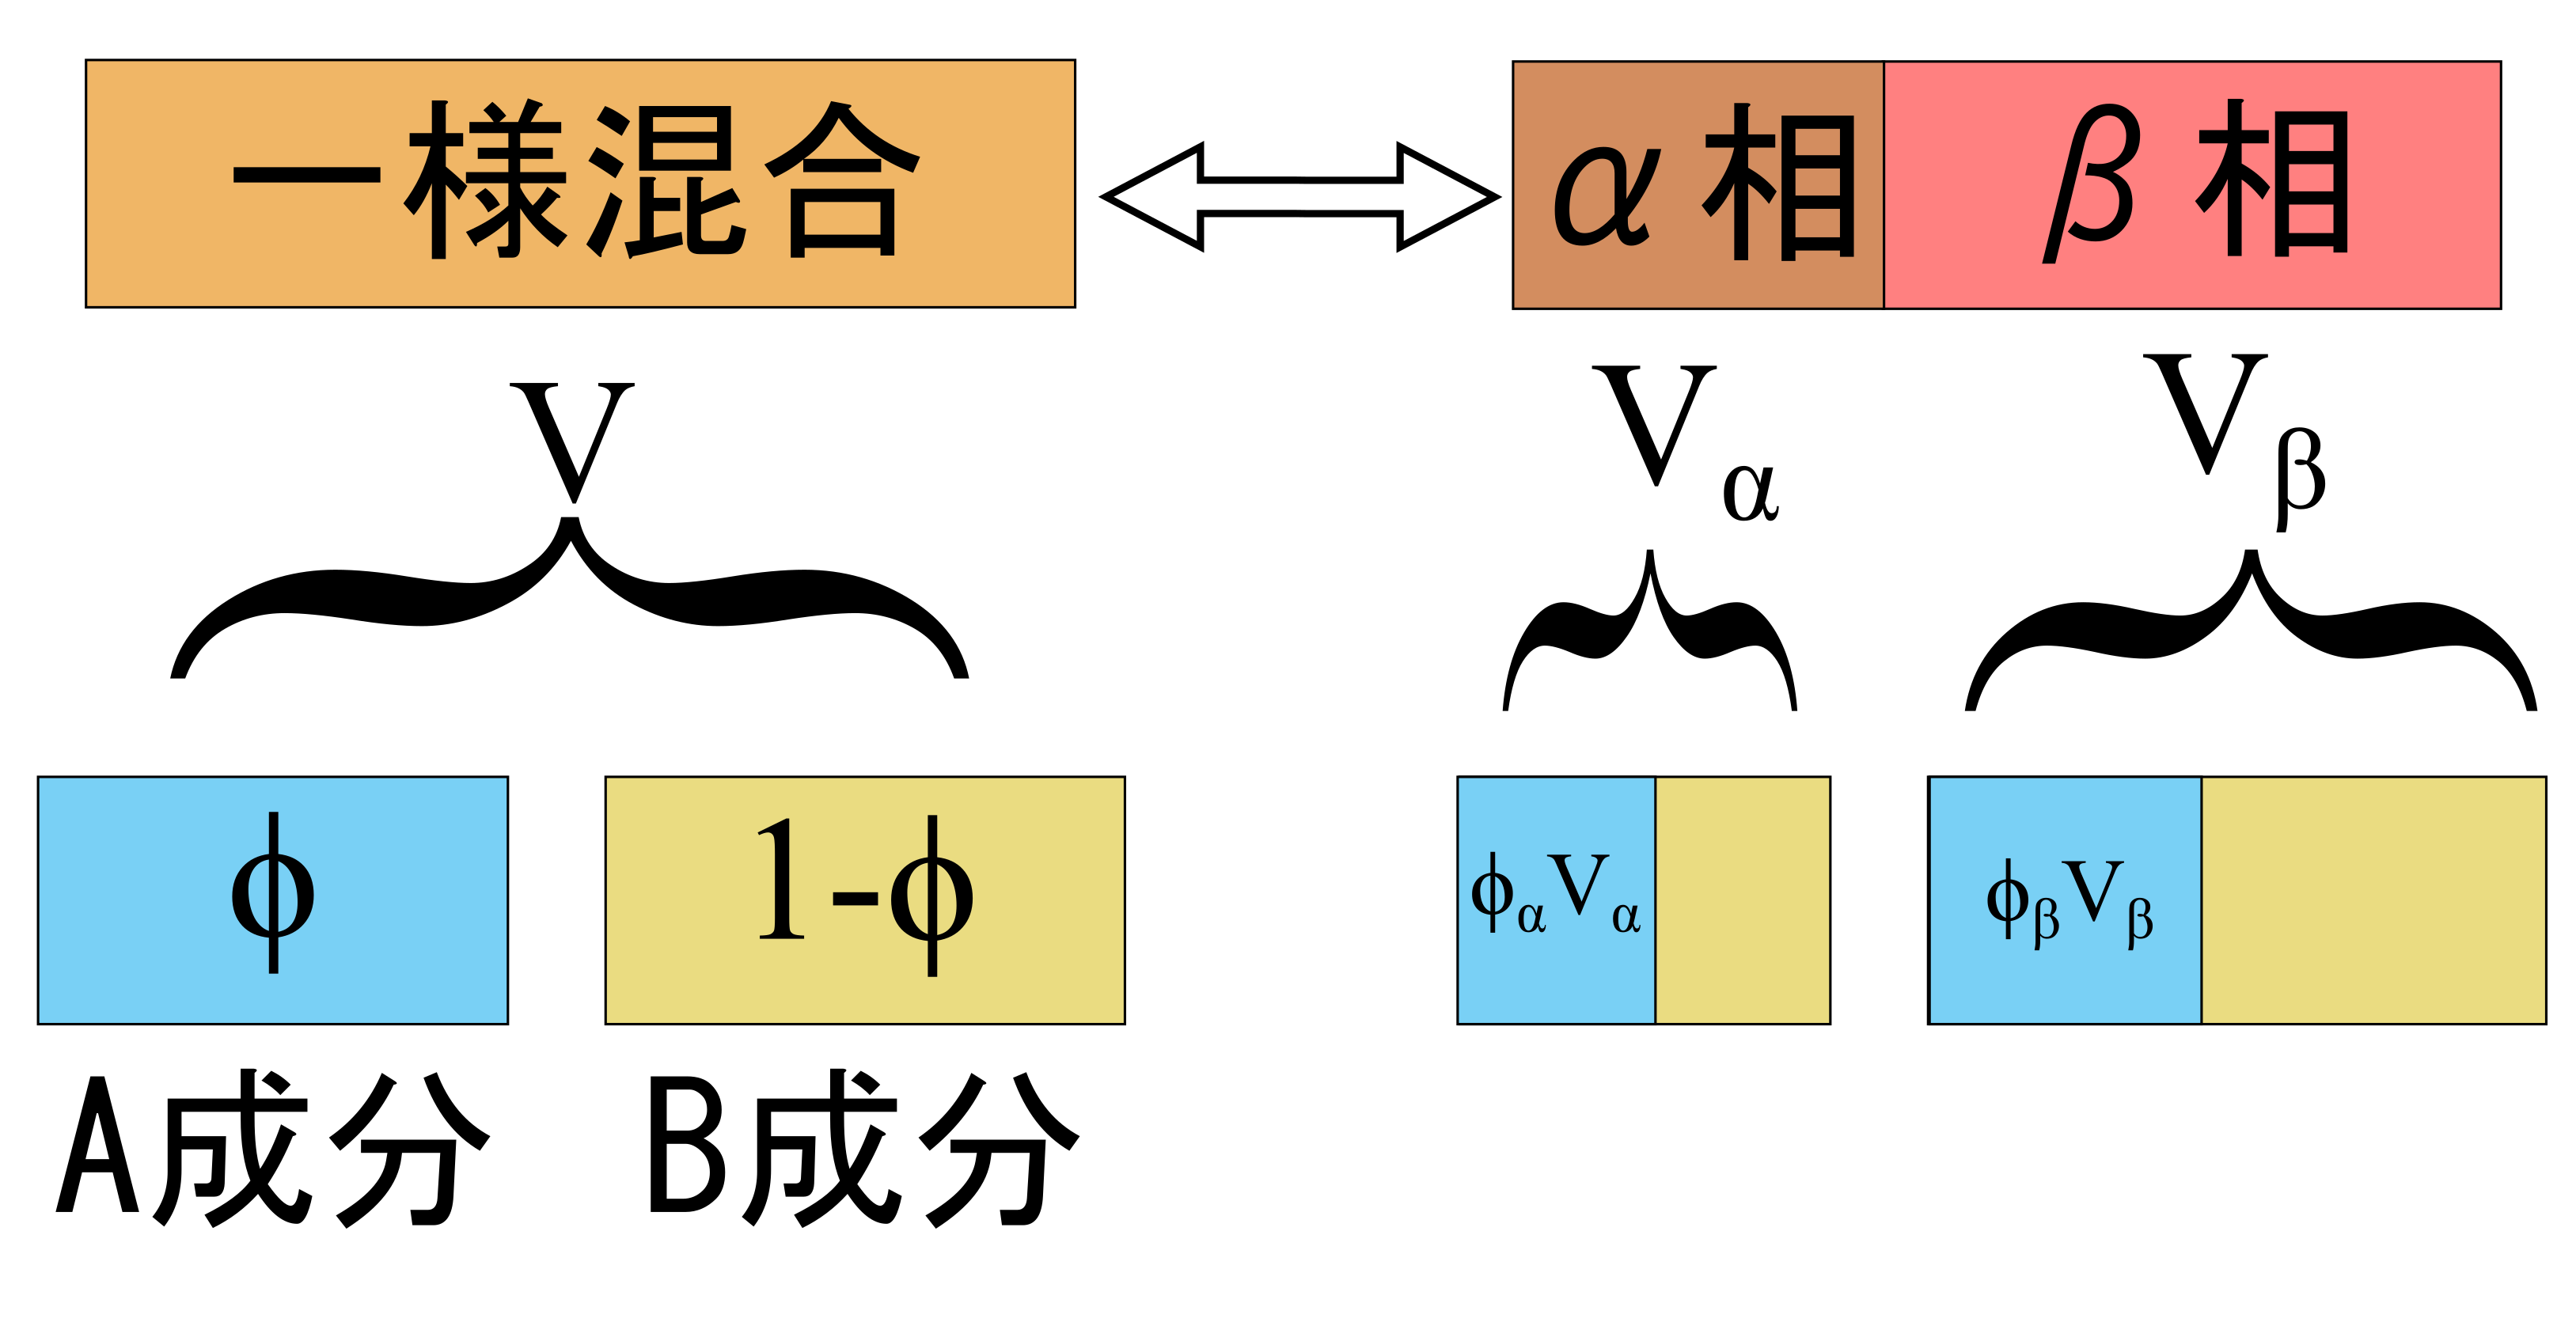
\includegraphics[width=.45\textwidth]{freeEform_1.png}
\end{frame}

\subsection{自由エネルギー密度曲線の形状による場合分け}
\begin{frame}
	\frametitle{自由エネルギー密度曲線の形状による場合分け}
		\begin{block}{下に凸な場合}
			\begin{columns}[c, onlytextwidth]
				\column{.6\linewidth}
					\begin{itemize}
						\item 局所的に$\phi _\alpha$ と $\phi _\beta$ に濃度ゆらぎが生じて相分離
						% \\(空間的な一箇所に注目)
						\item $f_{local}(\phi)$ は図中の赤い線上の値
						\item 一様状態の $f (\phi)$ と比べ\\
						$f_{local}(\phi) > f (\phi)$
						\item \alert{局所的な分離は自由エネルギー密度の上昇}
					\end{itemize}
				\column{.38\linewidth}
						\centering
							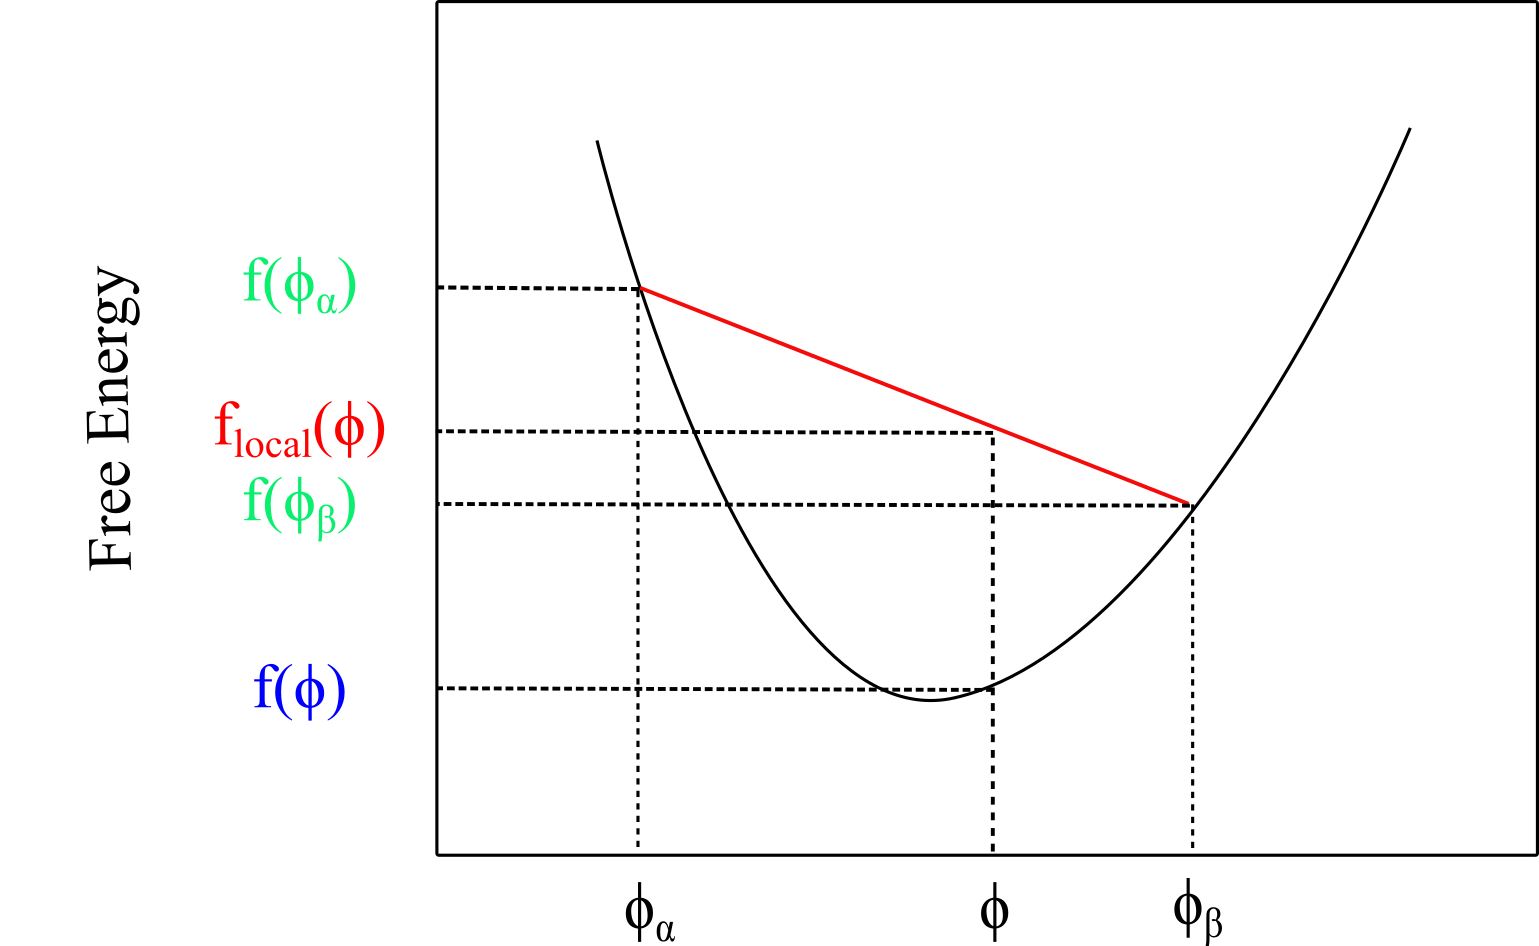
\includegraphics[width=\textwidth]{freeEform_2.png}
			\end{columns}
		\end{block}
 
		\begin{alertblock}{自由エネルギー密度曲線が下に凸な場合}
			\begin{itemize}
				\item 仕込み濃度のままで一様混合状態を維持する方が安定
				\item 相分離は生じない
			\end{itemize}
		\end{alertblock}
\end{frame}

\begin{frame}
	\frametitle{自由エネルギー密度曲線の形状による場合分け}
		\begin{block}{上に凸な場合}
			\begin{columns}[c, onlytextwidth]
				\column{.6\linewidth}
					\begin{itemize}
						% \item 局所的に$\phi _\alpha$ と $\phi _\beta$ に濃度ゆらぎが生じて相分離\\
						% (空間的な一箇所に注目)
						\item $f_{local}(\phi)$ は図中の赤い線上の値
						\item 一様状態の $f (\phi)$ と比べ\\
						$f_{local}(\phi) < f (\phi)$
						\item \alert{局所的に分離したほうが\\自由エネルギー密度が低下}
					\end{itemize}
				\column{.38\linewidth}
						\centering
							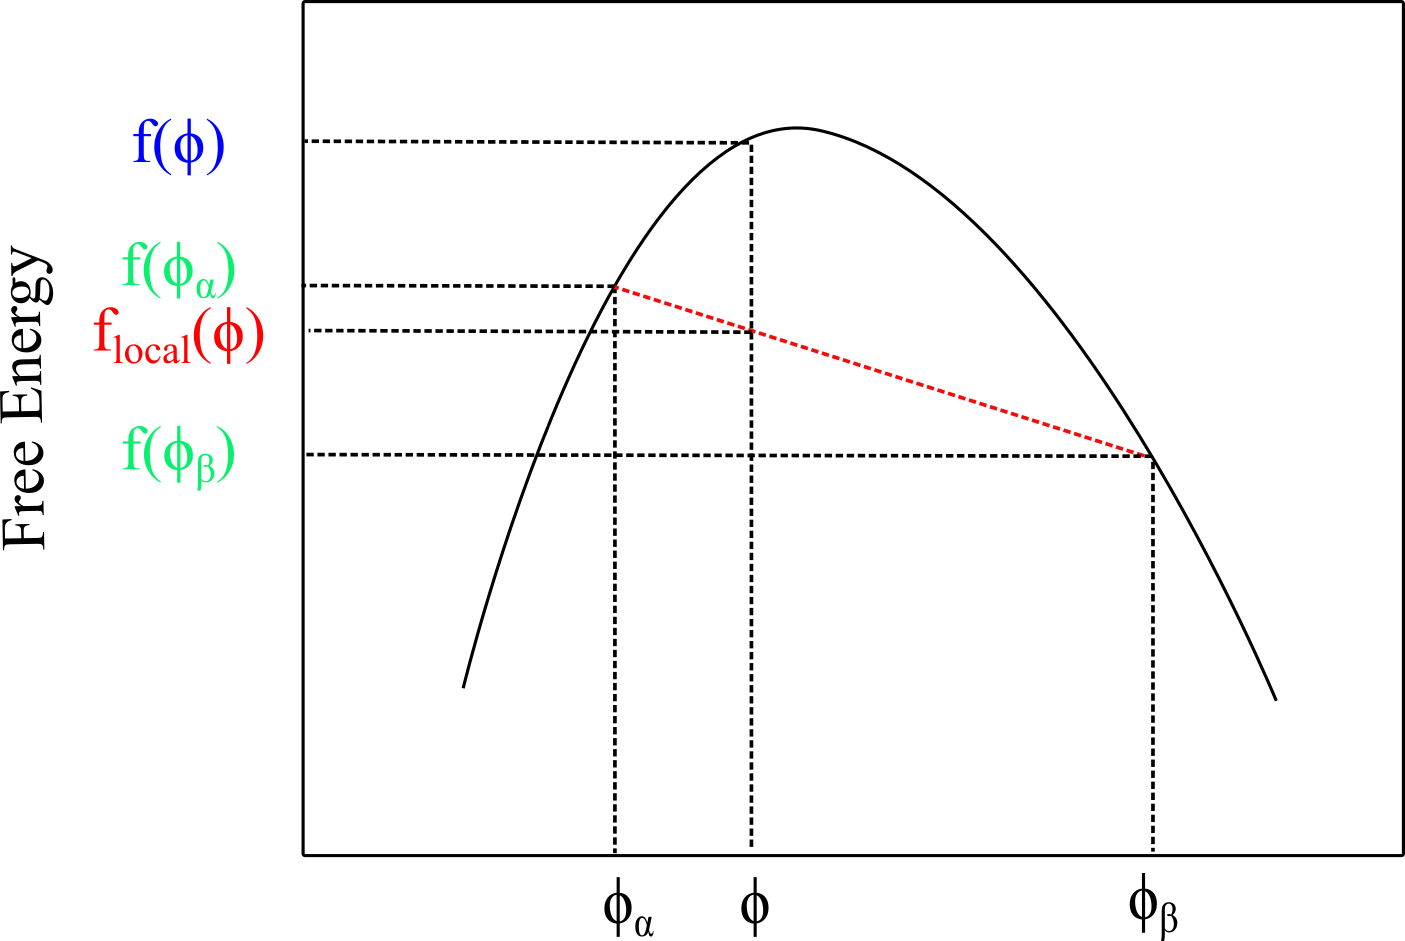
\includegraphics[width=\textwidth]{freeEform_3.png}
			\end{columns}
		\end{block}
 
		\begin{alertblock}{自由エネルギー密度曲線が上に凸な場合}
			\begin{itemize}
				\item ゆらぎが生じれば相分離することで安定化
				\item \alert{相分離は自発的}に生じる
				\item 理論上は\alert{互いの相にまったく溶解しない}
			\end{itemize}
		\end{alertblock}
\end{frame}

\begin{frame}
	\frametitle{共存組成について}
		\vspace{-3mm}
		\begin{block}{共存組成となる場合}
			\begin{columns}[c, onlytextwidth]
				\column{.58\linewidth}
					\begin{itemize}
						% \item ここまで示したように自由エネルギー曲線に上に凸な部分があればその領域で不安定化
						\item 自由エネルギー曲線の\alert{一部が上に凸}になった場合、
						\item 「自由エネルギー曲線上に\\おいて\alert{共通接線が引ける}」
					\end{itemize}
					\textcolor{blue}{導出の説明は省略}
				\column{.4\linewidth}
						\centering
							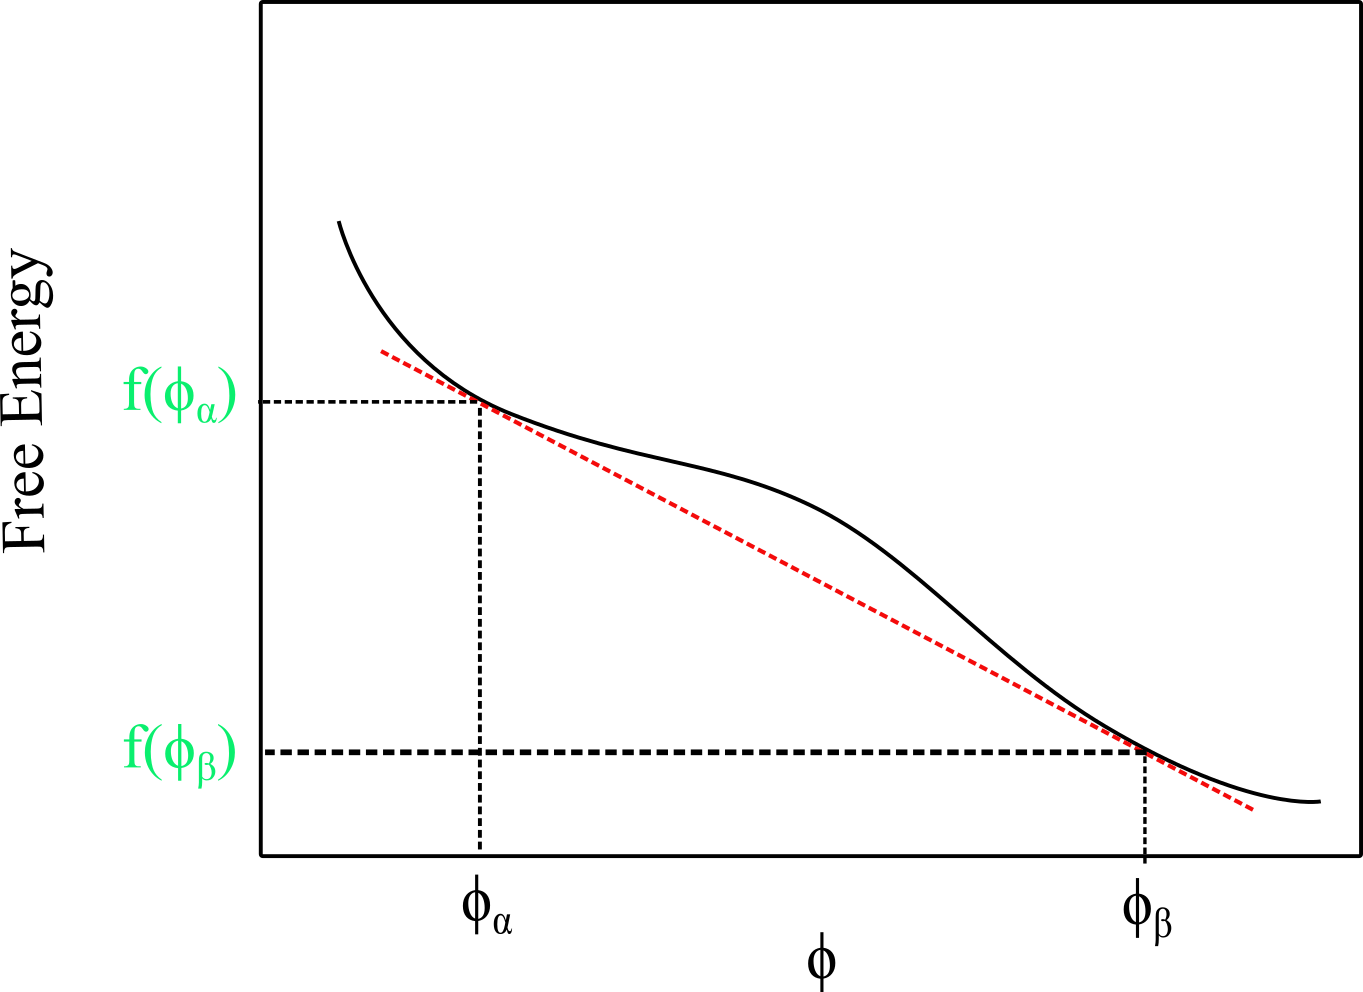
\includegraphics[width=.9\textwidth]{freeEform_4.png}
			\end{columns}
		\end{block}
		\vspace{-3mm}
		\begin{alertblock}{共存組成とは}
			\begin{columns}[c, onlytextwidth]
				\column{.58\linewidth}
				\begin{itemize}
					\item $\phi_\alpha < \phi  < \phi_\beta$ となる仕込みの体積分率 $\phi$ において、 
					\item $\alpha$ 相と $\beta$ 相中での成分 A の体積分率は、$\phi_\alpha$ および $\phi_\beta$
				\end{itemize}
				\column{.4\linewidth}
				\centering
				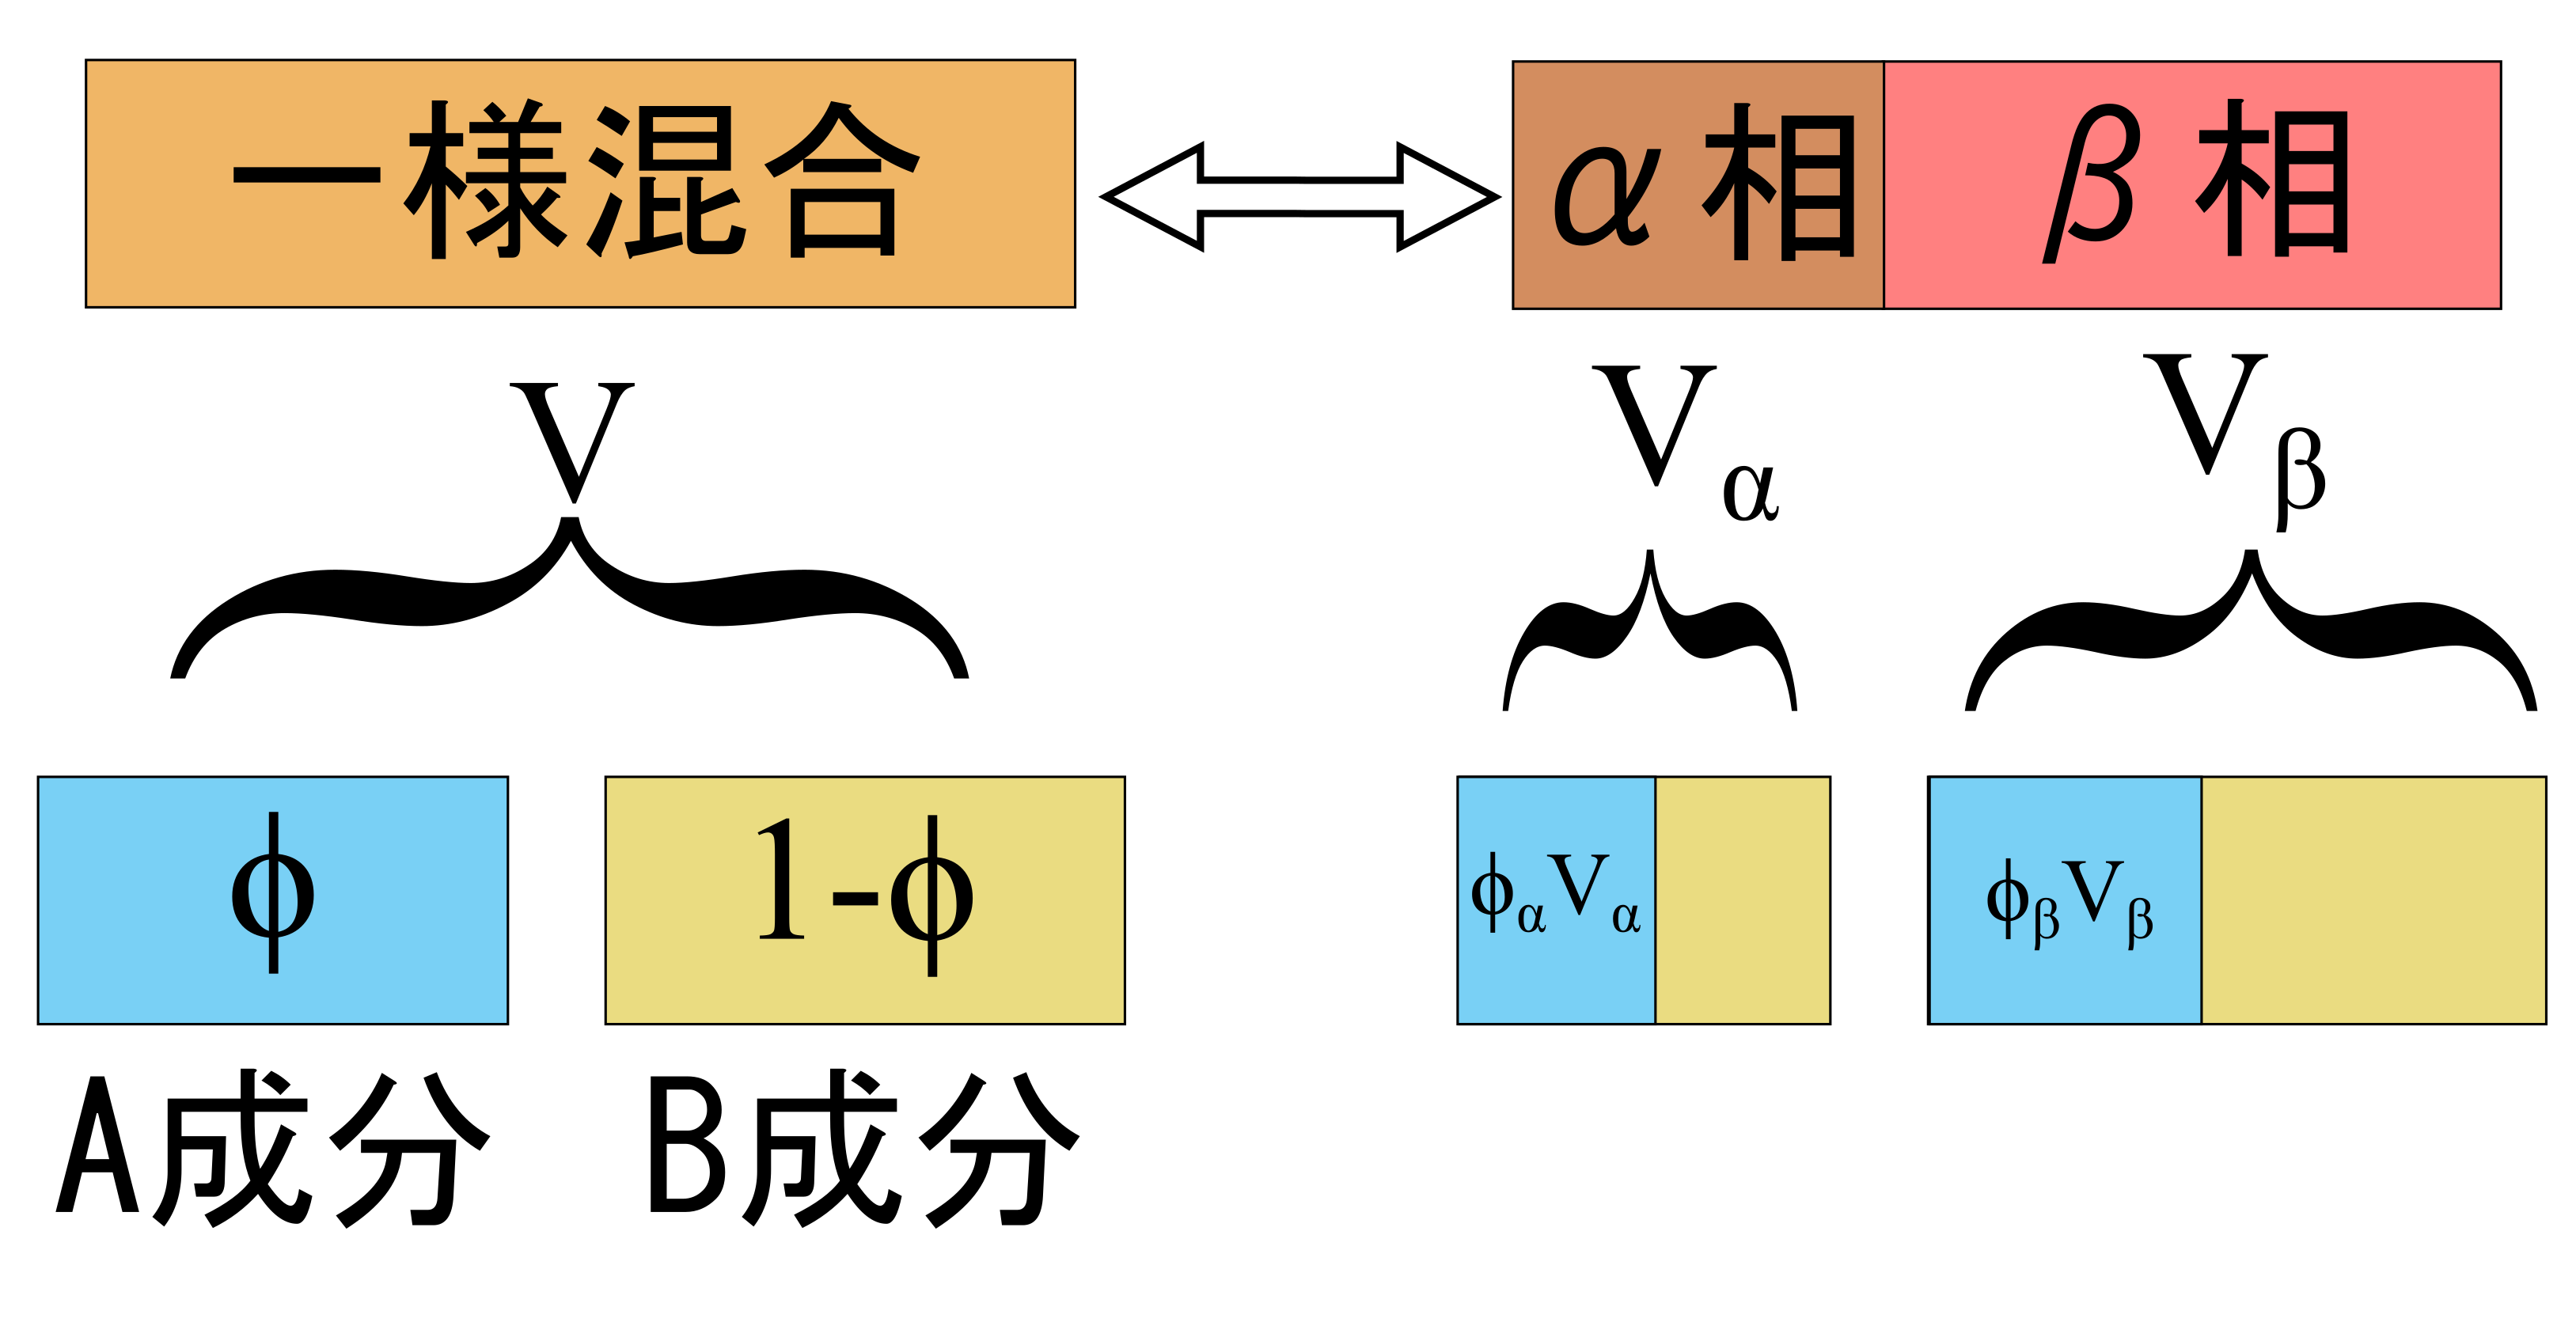
\includegraphics[width=\textwidth]{freeEform_1.png}
			\end{columns}
		\end{alertblock}
\end{frame}

\begin{frame}
	\frametitle{「混合状態と相図の理解」のまとめ}
        \begin{boxnote}
            \vspace{-3mm}
            \begin{itemize}
                \item 相溶と非相溶
                    \begin{itemize}
						\item 単純に溶ける溶けないの議論では不十分
                        \item 混合状態の詳細な理解には熱力学的考察が必要
                    \end{itemize}
				\item 自由エネルギーの濃度依存性について
                    \begin{itemize}
                        \item 自由エネルギーは $(\phi, f(\phi))$ 平面上の曲線
						\item 下に凸な場合⇔相分離は生じない
						\item 上に凸な場合⇔相分離は自発的に生じ、理論上は互いの相にまったく溶解しない
                        \item 自由エネルギー曲線の一部が上に凸
                        \begin{itemize}
							\item 共存組成となる
							\item 互いの相に一定量溶解して相分離
						\end{itemize}
                    \end{itemize} 
            \end{itemize}
        \end{boxnote}
\end{frame}


\end{document}